%  This is a LaTex file.

%  Homework for the course "AMath 585:  Applied Linear Algebra and Numerical Analysis", 
%  Autumn quarter, 2009, Anne Greenbaum.


%   A latex format for making homework assignments.


\documentclass[letterpaper,12pt]{article}

%          The page format, somewhat wider and taller page than in art12.sty.

\topmargin -0.1in \headsep 0in \textheight 8.9in \footskip 0.6in
\oddsidemargin 0in  \evensidemargin 0in  \textwidth 6.5in
\usepackage{graphicx}
\usepackage{listings}
\usepackage{caption}
\usepackage{subcaption}
\usepackage{color}
\usepackage{float}
\definecolor{keywords}{RGB}{255,0,90}
\definecolor{comments}{RGB}{0,0,113}
\definecolor{red}{RGB}{160,0,0}
\definecolor{green}{RGB}{0,150,0}
\definecolor{codegreen}{rgb}{0,0.6,0}
\definecolor{codegray}{rgb}{0.5,0.5,0.5}
\definecolor{codepurple}{rgb}{0.58,0,0.82}
\definecolor{backcolour}{rgb}{0.95,0.95,0.92}
\definecolor{brown}{rgb}{0.59, 0.29, 0.0}
\definecolor{beaublue}{rgb}{0.74, 0.83, 0.9}
\definecolor{orange}{rgb}{1.0, 0.5, 0.0}
\definecolor{darkslategray}{rgb}{0.18, 0.31, 0.31}
\definecolor{deepblue}{rgb}{0,0,0.5}
\definecolor{deepred}{rgb}{0.6,0,0}
\definecolor{deepgreen}{rgb}{0,0.5,0}
\lstdefinestyle{myMatlabstyle}{
	language=Matlab,
	backgroundcolor=\color{white},   
	commentstyle=\color{codegreen},
	keywordstyle=\color{blue},
	%identifierstyle=\color{brown},
	numberstyle=\tiny\color{codegray},
	stringstyle=\color{orange},
	basicstyle=\footnotesize,
	breakatwhitespace=false,         
	breaklines=true,                 
	captionpos=b,                    
	keepspaces=true,                 
	numbers=left,                    
	numbersep=5pt,                  
	showspaces=false,                
	showstringspaces=false,
	showtabs=false,                  
	tabsize=2
}
\lstdefinestyle{myPythonstyle}{
	language=Python, 
	basicstyle=\ttfamily\small, 
	keywordstyle=\color{blue},
	backgroundcolor=\color{white}, 
	commentstyle=\color{green},
	stringstyle=\color{red},
	showstringspaces=false,
	%identifierstyle=\color{brown},
	breaklines=true, 
}
\lstset{language=Matlab,frame=single}
\lstset{language=Python,frame=single}
\usepackage{amsmath}
\usepackage{epsfig}         % to insert PostScript figures
       % to insert PostScript figures

\begin{document}


%          Definitions of commonly used symbols.



%          The title and header.

\noindent
{\scriptsize AMath 585, Winter 2018} \hfill 

\begin{center}
\large
Assignment 5.
\normalsize

Jithin D. George, No. 1622555
\end{center}

\noindent
Due Friday, Feb. 16.
\vspace{.3in}


%           The questions!




\begin{enumerate}
\item
Write a code to solve Poisson's equation on the unit square with Dirichlet
boundary conditions:
\[
u_{xx} + u_{yy} = f(x,y) ,~~~0 < x,y < 1 
\]
\[
u(x,0) = u(x,1) = u(0,y) = u(1,y) = 1.
\]
Take $f(x,y) = x^2 + y^2$, and demonstrate numerically that your code 
achieves second order accuracy.  [Note:  If you do not know an analytic
solution to a problem, one way to check the code is to solve the problem
on a fine grid and pretend that the result is the exact solution, then
solve on coarser grids and compare your answers to the fine grid solution.
However, you must be sure to compare solution values corresponding to
the same points in the domain.]


{\bf Solution:}

\begin{figure}[H]

\centering
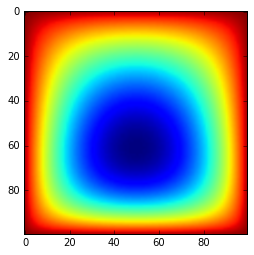
\includegraphics[width=0.25\textwidth]{plt5.png}



\end{figure}

	\begin{lstlisting}[style=myPythonstyle]
import numpy as np
import matplotlib.pyplot as plt
N = 12
a = -4*np.ones(N)
b = np.ones(N-1)
c = np.ones(N)
I = np.eye(N)
def tridiag(a, b, c, k1=-1, k2=0, k3=1):
    return np.diag(a, k1) + np.diag(b, k2) + np.diag(c, k3)
T = tridiag(b,a,b)
S = np.diag(b, -1)+ np.diag(b, 1)
A = np.kron(I,T)+np.kron(S,I )
def f(i,N):
    h = 1/(N+1) 
    x = (i%(N+1))*h
    g = int(i/N ) if i%N ==0 else int(i/N )+1
    y = g*h
    x = (i - (g-1)*N)*h
    return x**2 + y**2
fvec = np.array([])
for i in range(1,N**2+1):
    fvec = np.append(fvec,f(i,N**2))
h = 1/(N+1) 
i=0
for row in A:
    fvec[i]= fvec[i]*(h**2)+ sum(row)
    i+=1
fv = 6*(h**2)*fvec
x = np.linalg.solve(A, fvec)
xn = np.reshape(x,(N,N))
plt.imshow(xn)
print(np.linalg.norm(xn-x120[::10,::10], 2))

\end{lstlisting}


The infinity norm is used here. The solution at N = 120 is used as the 'accurate' solution.

\begin{tabular}{rr}
\hline
    N &      Error \\
\hline
 6  & 0.004582454\\
 12 & 0.001215613 \\
 24 & 0.000276484  \\
\hline
\end{tabular} 

The order seems to be O($h^2$).

\item
Now use the 9-point formula with the correction term described in Sec. 3.5 to solve
the same problem as in the previous exercise.
Again take $f(x,y) = x^2 + y^2$, and numerically test the order of accuracy of your code
by solving on a fine grid, pretending that is the exact solution, and comparing 
coarser grid approximations to the corresponding values of the fine grid solution.
Show what order of accuracy you achieve and try to explain why.

{\bf Solution:}

	\begin{lstlisting}[style=myPythonstyle]
import numpy as np
import matplotlib.pyplot as plt
N = 12
a = -20*np.ones(N)
b = 4*np.ones(N-1)
c = 4*np.ones(N)
d= np.ones(N-1)
I = np.eye(N)
def tridiag(a, b, c, k1=-1, k2=0, k3=1):
    return np.diag(a, k1) + np.diag(b, k2) + np.diag(c, k3)
T = tridiag(b,a,b)
R = tridiag(d,c,d)
S = tridiag(d,np.zeros(N),d)
A = np.kron(I,T)+np.kron(S,R)
def f(i,N):
    h = 1/(N+1) 
    x = (i%(N+1))*h
    g = int(i/N ) if i%N ==0 else int(i/N )+1
    y = g*h
    x = (i - (g-1)*N)*h
    return x**2 + y**2
fvec = np.array([])
for i in range(1,N**2+1):
    fvec = np.append(fvec,f(i,N**2)) + (h**2)/4
h = 1/(N+1) 
i=0

for row in A:
    fvec[i]= fvec[i]*6*(h**2)+ sum(row)
    i+=1
fv = 6*(h**2)*fvec
x = np.linalg.solve(A, fvec)
xn = np.reshape(x,(N,N))
plt.imshow(xn)
print(np.linalg.norm(xn-x120[::10,::10], 2))

\end{lstlisting}

The infinity norm is used here. The solution at N = 120 is used as the 'accurate' solution.

\begin{tabular}{rr}
\hline
    N &      Error \\
\hline
 6  & 5.10230545e-05\\
 12 & 3.17394091e-06 \\
 24 & 1.99308866e-07  \\
\hline
\end{tabular} 

The order seems to be O($h^4$).
\item 

We have discussed using finite element methods to solve elliptic PDE's such as 
\[
\bigtriangleup u = f~~\mbox{ in } \Omega ,~~~u = 0~~\mbox{ on } \partial \Omega ,
\]
with {\em homogeneous} Dirichlet boundary conditions.  How could you modify the procedure
to solve the {\em inhomogeneous} Dirichlet problem:
\[
\bigtriangleup u = f~~\mbox{ in } \Omega ,~~~u = g~~\mbox{ on } \partial \Omega ,
\]
where $g$ is some given function?  Derive the equations that you would need to
solve to compute, say, a continuous piecewise bilinear approximation for this problem
when $\Omega$ is the unit square $(0,1) \times (0,1)$.

{\bf Solution:}

\item
The key to efficiency in the \verb+chebfun+ package, which you used in a previous homework
exercise, is the ability to rapidly translate between the values of a function at the
Chebyshev points, $\cos ( \pi j/n )$, $j=0, \ldots , n$, and the coefficients $a_0 , \ldots , a_n$,
in a Chebyshev expansion of the function's $n$th-degree polynomial interpolant:
$p(x) = \sum_{j=0}^n a_j T_j (x)$, where $T_j (x) = \cos ( j \arccos (x) )$ is the $j$th
degree Chebyshev polynomial.  Knowing the coefficients $a_0 , \ldots , a_n$, one can evaluate
$p$ at the Chebyshev points by evaluating the sums
\begin{equation}
p ( \cos ( k \pi / n ) ) = \sum_{j=0}^n a_j \cos ( j k \pi / n ) ,~~~k=0, \ldots , n.
\label{Cheby}
\end{equation}
These sums are much like the real part of the sums in the FFT,
\[
F_k = \sum_{j=0}^{n-1} e^{2 \pi i j k / n} f_j ,~~~k=0, \ldots , n-1 ,
\]
but the argument of the cosine differs by a factor of $2$ from the values that would make
them equal.  Explain how the FFT or a closely related procedure could be used to evaluate
the sums in (\ref{Cheby}).  To go in the other direction, and efficiently determine the coefficients
$a_0 , \ldots , a_n$ from the function values $f( \cos ( k \pi / n ) )$, what method would you use?


{\bf Solution:}

\[2 * p ( \cos ( k \pi / n ) ) = 2 \sum_{j=0}^n a_j \cos ( j k \pi / n ) \]
\[= \sum_{j=0}^n a_j \cos ( j k \pi / n ) + \sum_{j=0}^n a_j \cos ( j k \pi / n ) \]
\[= \sum_{j=0}^n a_j \cos ( j k \pi / n ) + \sum_{j=0}^n a_j \cos ( (n+j) k \pi / n ) \]
\[= \sum_{j=0}^{2n-1} a_j \cos ( j k \pi / n ) + a_0 +a_n \cos ( k \pi ) \]
\[= \sum_{j=0}^{2n-1} a_j \cos ( j k \pi / n ) + a_0 +a_n (-1)^k \]
\[= Re(\sum_{j=0}^{2n-1} a_j e^{ j k \pi / n  }) + a_0 +a_n (-1)^k \]
Thus, 
\[ p ( \cos ( k \pi / n ) ) = \frac{1}{2} (Re(\sum_{j=0}^{2n-1} a_j e^{ j k \pi / n  }) + a_0 +a_n (-1)^k) \]
The first term can be calculated using the FFT
\[ p ( k) = \frac{1}{2} (Re(\sum_{j=0}^{2n-1} a_j e^{ j k \pi / n  }) + a_0 +a_n (-1)^k) \]
\[ \sum_{k=0}^n 2p ( k) = \sum_{k=0}^n  Re(\sum_{j=0}^{2n-1} a_j e^{ j k \pi / n  }) +  \sum_{k=0}^n  a_0 + \sum_{k=0}^n a_n (-1)^k \]
\[ \sum_{k=0}^n 2 p ( k) = \sum_{k=0}^n  Re(\sum_{j=0}^{2n-1} a_j e^{ j k \pi / n  }) +  p(0)+ p(n)\]
\[ p (0) +\sum_{k=1}^{n-1} 2 p ( k) + p(n) = \sum_{k=0}^n  \sum_{j=0}^{2n-1} a_j Re(e^{ j k \pi / n  }) \]
\[ p (0) +\sum_{k=1}^{n-1} 2 p ( k) + p(n) = \sum_{j=0}^{2n-1}  \sum_{k=0}^n  a_j Re(e^{ j k \pi / n  }) \]
We can see that
\[ p (0)  = \sum_{j=0}^{2n-1}  \sum_{k=0}^n  a_j  \]
\[ p (n)  = \sum_{j=0}^{2n-1}  \sum_{k=0}^n  a_j (-1)^n \]
This looks like values obtained after a DFT.
Thus, taking the ifft of the vector (p(0), p(1),p(2), ...p(n-1), p(n), p(n-1),p(n-2),..., p(2),p(1)) can get you back the coefficients $a_n$
\end{enumerate}

\end{document}
